\documentclass[11pt,a4paper]{article}
\usepackage[utf8]{inputenc}
\usepackage{microtype}
\usepackage[margin=2.2cm]{geometry}
\usepackage{xcolor,booktabs,longtable,array,tabularx,float,enumitem,caption}
\usepackage{tikz}
\usetikzlibrary{positioning,arrows.meta,shapes.geometric,patterns,calc,fit,backgrounds}
\usepackage{pgfplots}\pgfplotsset{compat=1.16}
\usepackage[hidelinks]{hyperref}
\definecolor{unmblue}{HTML}{1F4E79}\definecolor{accent}{HTML}{C55A11}\definecolor{soft}{HTML}{DEEAF6}
\definecolor{c1}{HTML}{9DC3E6}\definecolor{c2}{HTML}{2E75B6}\definecolor{c3}{HTML}{1F4E79}\definecolor{c4}{HTML}{BFBFBF}
\setlist{nosep,leftmargin=1.4em}
\newcommand{\um}{\,\ensuremath{\mu}m}
\newcommand{\flag}[1]{\textcolor{accent}{\textbf{#1}}}
\title{\textbf{Microplastic Size in Rivers and Ponds, and the University of Nottingham Malaysia Contribution}\\[2pt]\large Literature screen of the filtered Bibliometrix dataset}
\author{Group Project -- Case Studies (Combined)}
\date{\today}
\begin{document}
\maketitle

\begin{abstract}\noindent
This report answers two questions from the uploaded Bibliometrix dataset (\texttt{Bibliometrix\_\allowbreak Filtered.RData}): (1) what microplastic size is most commonly reported in rivers and ponds, with a focus on the Semenyih River; and (2) which papers are affiliated with the University of Nottingham Malaysia (UNM), what methods they used, and what they found. Every count below comes from a documented filter applied to the records in the file, and the filter code and output tables are included in the package. In the screened river/lake/pond abstracts that state a dominant size class (n\,=\,@@N6@@), about @@SUBMM_A@@\% report a class below 1\,mm. UNM contributes nine records, of which five are primary microplastic studies in the Langat--Semenyih catchment. \flag{Important limit:} the dataset contains titles, abstracts and metadata only, so instrument models and accuracy (recovery) rates are mostly not recoverable from it and are flagged for full-text extraction.
\end{abstract}

\section{Data provenance and the 10,833 vs 10,897 discrepancy}
The uploaded file contains one data frame (\texttt{M}) with @@N0@@ records and 68 fields. You mentioned 10,833 papers; I could not reproduce that figure from this file (e.g.\ de-duplicating on DOI gives 10,890 and removing records without an abstract gives @@N1@@). All counts here therefore start from @@N0@@ records, and the funnel shows every step so the base can be adjusted if a different starting set is intended. Of the records, 8,800 originate from Web of Science and 2,097 from Scopus.

\section{How the papers were filtered}
\subsection{Funnel for Question 1 (size in rivers and ponds)}
Filters were applied to the concatenated title, abstract and author keywords (upper-cased, micro sign normalised). Exact patterns are in Appendix~\ref{app:rules} and in \texttt{scripts/filter\_pipeline.py}.

\begin{figure}[H]\centering
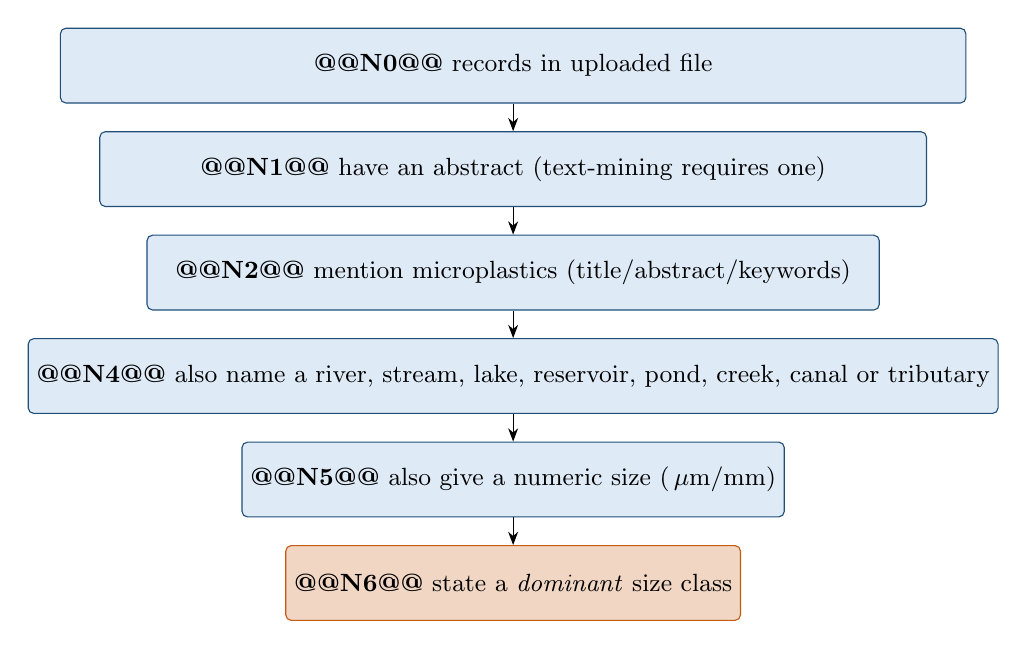
\begin{tikzpicture}[font=\small,
  box/.style={draw=unmblue,fill=soft,rounded corners=2pt,minimum height=0.95cm,align=center,inner sep=3pt}]
\node[box,minimum width=11.5cm] (a) at (0,0) {\textbf{@@N0@@} records in uploaded file};
\node[box,minimum width=10.5cm,below=0.35cm of a] (b) {\textbf{@@N1@@} have an abstract (text-mining requires one)};
\node[box,minimum width=9.3cm,below=0.35cm of b] (c) {\textbf{@@N2@@} mention microplastics (title/abstract/keywords)};
\node[box,minimum width=7.6cm,below=0.35cm of c] (d) {\textbf{@@N4@@} also name a river, stream, lake, reservoir, pond, creek, canal or tributary};
\node[box,minimum width=5.6cm,below=0.35cm of d] (e) {\textbf{@@N5@@} also give a numeric size (\um/mm)};
\node[box,minimum width=4.2cm,fill=accent!25,draw=accent,below=0.35cm of e] (f) {\textbf{@@N6@@} state a \emph{dominant} size class};
\foreach \x/\y in {a/b,b/c,c/d,d/e,e/f}{\draw[-{Stealth}] (\x) -- (\y);}
\end{tikzpicture}
\caption{Filter funnel for Question 1. A broader ``freshwater/wetland'' wording would keep @@N3@@ records at the water-body step; it was not used because it admits non-river/pond systems.}
\end{figure}

How the last step works: for each abstract that passed the numeric-size step, sentences were kept only if they contained a dominance word (dominant, majority, most, predominant, mainly, prevalent, etc.) and a size expression. Sentences that merely define microplastics ($<$5\,mm, 1\um--5\,mm) or give a study's search range were removed. The first remaining expression was converted to millimetres and assigned a class by its \emph{upper bound}: $\le$0.1\,mm, 0.1--0.5\,mm, 0.5--1\,mm (this class also holds generic ``$<$1\,mm'' statements) and $>$1\,mm up to 5\,mm.

\subsection{Filter for Question 2 (University of Nottingham Malaysia)}
Six affiliation fields (\texttt{C1}, \texttt{affiliations}, \texttt{AU\_UN}, \texttt{RP}, \texttt{AU1\_UN}, \texttt{organization}) were searched for ``Nottingham'' within 80--200 characters of ``Malaysia'', ``Semenyih'', ``Broga'' or ``Selangor'', plus the abbreviation UNMC. This returned \textbf{9 records}. For comparison, 33 records mention Nottingham in \texttt{C1}, but most belong to the UK campus, Nottingham Ningbo China, Nottingham Trent University or the British Geological Survey, and were excluded. A cross-check on author names (Chen HL, Selvam SB, Gibbins C, Ting KN, Ng YS, Show PL) found two further records not in the set: a Ningbo-campus review and an unrelated schlieren-imaging paper; neither lists a Malaysian Nottingham address.

\section{Question 1 -- Literature review: common microplastic size in rivers and ponds}
\subsection{What the screen shows}
Among the @@N6@@ river/lake/pond abstracts that state a dominant class, sub-millimetre particles dominate (Figure~\ref{fig:bars}). Classes by share: $<$100\um{} @@PA1@@\%, 100--500\um{} @@PA2@@\%, 0.5--1\,mm @@PA3@@\%, and 1--5\,mm @@PA4@@\% (counts @@CNT1@@, @@CNT2@@, @@CNT3@@, @@CNT4@@). The pattern is similar in rivers (n\,=\,@@NR@@; @@SUBMM_R@@\% sub-millimetre), lakes and reservoirs (n\,=\,@@NL@@; @@SUBMM_L@@\%) and ponds (n\,=\,@@NP@@; @@SUBMM_P@@\%, small sample so indicative only). The abstracts also report that fibres are usually the dominant shape in rivers.

\begin{figure}[H]\centering
\begin{tikzpicture}
\begin{axis}[ybar,width=15.5cm,height=7.2cm,bar width=9pt,ymin=0,ymax=55,ylabel={Share of papers (\%)},
 symbolic x coords={lt100,100to500,500to1000,1to5},xtick=data,
 xticklabels={$<$100\um,100--500\um,0.5--1\,mm,1--5\,mm},enlarge x limits=0.15,
 legend style={at={(0.5,1.02)},anchor=south,legend columns=4,font=\small,draw=none},
 nodes near coords,every node near coord/.append style={font=\tiny,rotate=90,anchor=west},
 tick label style={font=\small}]
\addplot[fill=c3,draw=c3] coordinates {@@C_ALL@@};
\addplot[fill=c2,draw=c2] coordinates {@@C_RIV@@};
\addplot[fill=c1,draw=c1] coordinates {@@C_LAK@@};
\addplot[fill=accent!70,draw=accent] coordinates {@@C_POND@@};
\legend{All (n=@@NA@@),River (n=@@NR@@),Lake/reservoir (n=@@NL@@),Pond (n=@@NP@@)}
\end{axis}
\end{tikzpicture}
\caption{Dominant size class reported in abstracts (river/lake/pond microplastic papers). A paper can appear in more than one water-body group.}\label{fig:bars}
\end{figure}

\subsection{Why the answer depends on the method}
Reported size is partly a function of what the method can see. Within the UNM group's own fish/invertebrate study, visual inspection covered 0.1--5\,mm while a new automated method covered 0.004--0.1\,mm and returned substantially higher counts, so visual work under-estimates small particles \cite{ng24}. A Perak River study using fluorescence and FTIR microscopy found most particles at 1--10\um{} \cite{hassan25}, and a review of Malaysian rivers notes that detection limits fell to 1--10\um{} as the field moved from visual microscopy to $\mu$FTIR and Py-GC/MS \cite{bouida26}. The headline ``most are below 1\,mm'' is therefore robust, but the split between 100--500\um{} and 0.5--1\,mm depends on mesh and instrument.

\subsection{Malaysian and pond examples from the screen}
\begin{table}[H]\centering\small
\begin{tabularx}{\textwidth}{@{}p{3.6cm}p{3.8cm}X@{}}
\toprule Study & Water body & Dominant size stated in abstract \\\midrule
Zaki et al.\ 2024 \cite{zaki24} & Selangor River, water & 600--1000\um{} (26.3\%); fibres 64.3\%; stereomicroscope + FTIR \\
Zaki et al.\ 2023 \cite{zaki23} & Selangor River, sediment & $<$300\um{} (more than half of particles) \\
Ali et al.\ 2025 \cite{ali25} & Langat River & 10--1000\um{}; mostly fragments \\
Anuar et al.\ 2023 \cite{anuar23} & Langat and Kelantan & Sizes classified; values not in abstract; $\mu$FTIR, Py-GC/MS, SEM-EDS \\
Sheriff and Adams 2026 \cite{sheriff26} & Review, Malaysia & Langat particles often below 1\,mm \\
Hassan et al.\ 2025 \cite{hassan25} & Perak River intake & Mostly 1--10\um{} (fluorescence/FTIR microscopy) \\
Cherating River 2020 \cite{cherating20} & River + mangrove & Fragments 0.5--1.0\,mm \\
Klang estuary 2021 \cite{klang21} & Estuary water & 300--1000\um{} \\
Baram estuary 2021 \cite{baram21} & Estuary & 0.3--1\,mm \\
Urban ponds, Raipur 2024 \cite{raipur24} & 20 tropical ponds, India & 500--1000\um{} class prevailing \\
\bottomrule\end{tabularx}
\caption{Selected regional and pond studies. Values are taken from abstracts only.}
\end{table}

\section{Question 1.1 -- Focus diagram: microplastic size in the Semenyih River}
\flag{What the dataset can and cannot say.} The only Semenyih-specific study in the file is Chen et al.\ 2023 (UNM), which sampled eight sites on the upper Semenyih River, with five replicate water and bed samples on each of three dates (160 samples), and found microplastics in every sample: $3.12\pm2.49$ particles/L in water and $6027\pm16{,}586$ particles/m$^{2}$ on the bed, with fibres dominant in both \cite{chen23}. Its abstract does \emph{not} give a size histogram. The diagram therefore places the Semenyih evidence in the context of the neighbouring Langat and Selangor basin results and the size windows of the UNM group's own methods. The Semenyih River drains to the Langat, which the UNM team also sampled \cite{chen21a}.

\begin{figure}[H]\centering
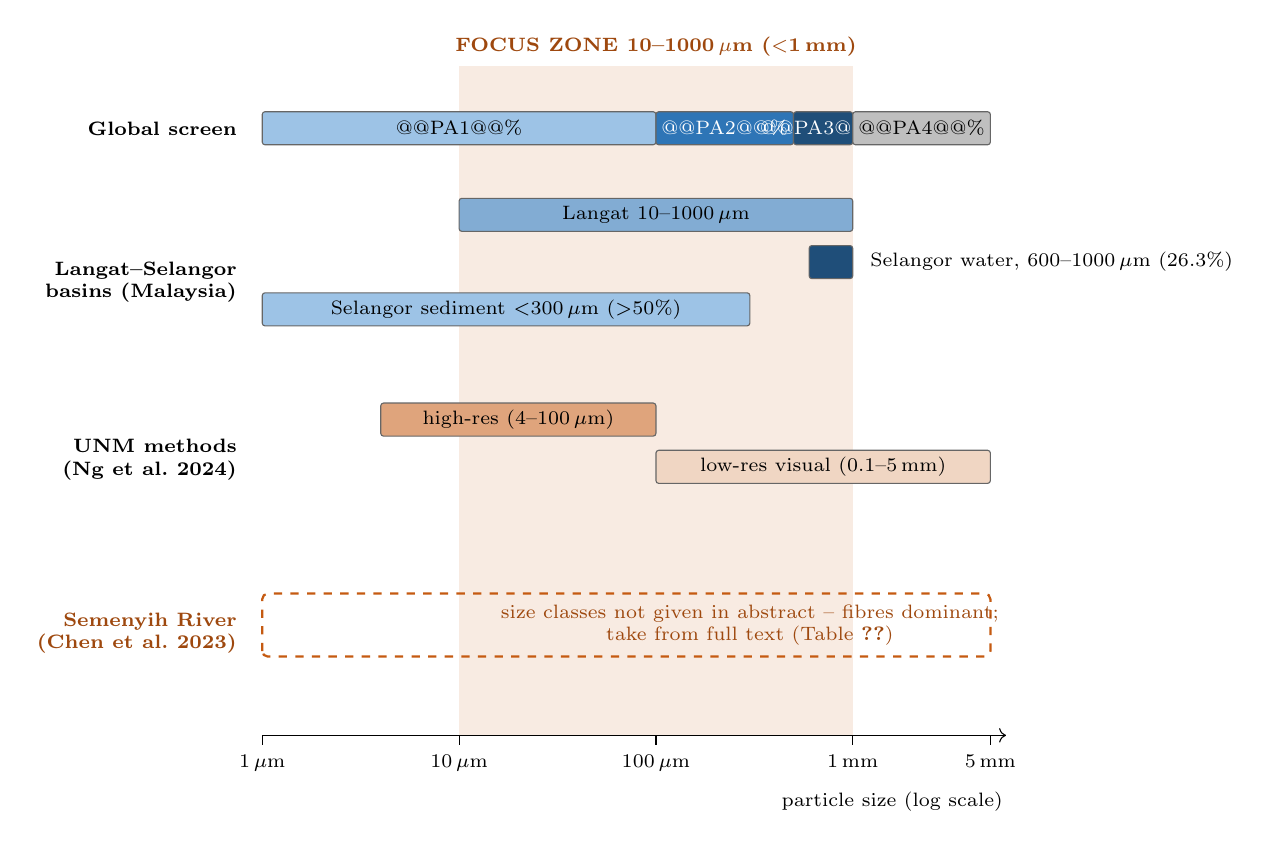
\begin{tikzpicture}[font=\footnotesize]
\def\sx{2.5}
\newcommand{\rbar}[6]{%
 \pgfmathsetmacro{\xa}{ln(#1)/ln(10)*\sx}\pgfmathsetmacro{\xb}{ln(#2)/ln(10)*\sx}%
 \draw[fill=#4,draw=black!60,rounded corners=1pt] (\xa,#3) rectangle (\xb,#3+0.42);
 \node[font=\scriptsize,#6] at ({(\xa+\xb)/2},#3+0.21) {#5};}
% focus zone 10-1000 um
\pgfmathsetmacro{\fa}{1*\sx}\pgfmathsetmacro{\fb}{3*\sx}
\fill[accent!12] (\fa,-0.3) rectangle (\fb,8.2);
\node[accent!80!black,font=\scriptsize\bfseries,anchor=south] at ({(\fa+\fb)/2},8.2) {FOCUS ZONE 10--1000\um\ ($<$1\,mm)};
% axis
\draw[->] (0,-0.3) -- ({ln(6000)/ln(10)*\sx},-0.3);
\foreach \v/\l in {1/1\um,10/10\um,100/100\um,1000/1\,mm,5000/5\,mm}{
 \pgfmathsetmacro{\tx}{ln(\v)/ln(10)*\sx}\draw (\tx,-0.3)--(\tx,-0.42);\node[anchor=north,font=\scriptsize] at (\tx,-0.42){\l};}
\node[anchor=north,font=\scriptsize] at ({3.2*\sx},-0.9) {particle size (log scale)};
% row labels
\node[anchor=east,align=right,font=\scriptsize\bfseries] at (-0.2,7.4) {Global screen};
\node[anchor=east,align=right,font=\scriptsize\bfseries] at (-0.2,5.45) {Langat--Selangor\\basins (Malaysia)};
\node[anchor=east,align=right,font=\scriptsize\bfseries] at (-0.2,3.2) {UNM methods\\(Ng et al.\ 2024)};
\node[anchor=east,align=right,font=\scriptsize\bfseries,text=accent!80!black] at (-0.2,1.0) {Semenyih River\\(Chen et al.\ 2023)};
% global
\rbar{1}{100}{7.2}{c1}{\scriptsize @@PA1@@\%}{text=black}
\rbar{100}{500}{7.2}{c2}{\scriptsize @@PA2@@\%}{text=white}
\rbar{500}{1000}{7.2}{c3}{\scriptsize @@PA3@@\%}{text=white}
\rbar{1000}{5000}{7.2}{c4}{\scriptsize @@PA4@@\%}{text=black}
% Malaysia
\rbar{10}{1000}{6.1}{c2!60}{Langat 10--1000\um}{text=black}
\rbar{600}{1000}{5.5}{c3}{}{text=white}
\node[anchor=west,font=\scriptsize] at ({ln(1000)/ln(10)*\sx+0.1},5.71) {Selangor water, 600--1000\um\ (26.3\%)};
\rbar{1}{300}{4.9}{c1}{Selangor sediment $<$300\um\ ($>$50\%)}{text=black}
% UNM windows
\rbar{4}{100}{3.5}{accent!55}{high-res (4--100\um)}{text=black}
\rbar{100}{5000}{2.9}{accent!25}{low-res visual (0.1--5\,mm)}{text=black}
% Semenyih unknown
\draw[dashed,accent,thick,rounded corners=2pt] ({ln(1)/ln(10)*\sx},0.7) rectangle ({ln(5000)/ln(10)*\sx},1.5);
\node[font=\scriptsize,align=center,text=accent!80!black] at ({ln(300)/ln(10)*\sx},1.1) {size classes not given in abstract -- fibres dominant;\\take from full text (Table~\ref{tab:fill})};
\end{tikzpicture}
\caption{Focus diagram. Top row: share of the @@NA@@ screened papers by dominant class. Middle: dominant classes reported for the neighbouring Langat and Selangor basins \cite{ali25,zaki24,zaki23}. Orange: size windows of the UNM group's low- and high-resolution methods \cite{ng24}. Bottom: the Semenyih River study \cite{chen23}, whose size distribution must be filled from the full paper. The shaded zone marks where the regional evidence concentrates.}\label{fig:focus}
\end{figure}

\noindent\textbf{Reading the diagram.} All regional evidence concentrates below 1\,mm, with water samples centred around 0.3--1\,mm and sediment skewed finer ($<$300\um). Because the UNM group's own work shows that a visual method misses the finest particles \cite{ng24}, the Semenyih size distribution should be read as a lower bound on the fine fraction. Table~\ref{tab:fill} lists what to extract from the full text of the Semenyih paper to complete the diagram.

\begin{table}[H]\centering\small
\begin{tabularx}{\textwidth}{@{}lXl@{}}
\toprule Item to extract (Chen et al.\ 2023 \cite{chen23}) & Why it is needed & Value \\\midrule
Size-class table, water (\% per class) & Replaces the dashed box with real bars & \emph{to fill} \\
Size-class table, bed sediment & Water vs bed comparison (fragments rose on the bed) & \emph{to fill} \\
Smallest size counted / mesh & Sets the lower edge of the bar & \emph{to fill} \\
Identification instrument and blank/recovery tests & Needed for Section~\ref{sec:method} accuracy column & \emph{to fill} \\
\bottomrule\end{tabularx}
\caption{Items to complete the Semenyih size bars.}\label{tab:fill}
\end{table}

\section{Question 2 -- Papers affiliated with University of Nottingham Malaysia}
\begin{table}[H]\centering\scriptsize
\begin{tabularx}{\textwidth}{@{}p{1.1cm}p{0.8cm}Xp{3.0cm}p{0.8cm}p{2.4cm}@{}}
\toprule Ref. & Year & Title & Journal & Cites & Role in this review \\\midrule
@@UNMROWS@@
\bottomrule\end{tabularx}
\caption{The nine records returned by the UNM affiliation filter (citation counts are the \texttt{TC} field in the dataset).}
\end{table}
Five records are primary microplastic studies (river monitoring, source apportionment, biota and image analysis); one is the group's Southeast Asia review. The three others carry a UNM address through the Department of Chemical and Environmental Engineering (Show PL) and cover marine/health reviews, phytoplankton and a Taiwan-led aging and sorption experiment, so they are less relevant to river detection.

\subsection{Methodology for detecting microplastics, UNM equipment and accuracy}\label{sec:method}
\flag{Limitation.} Abstracts rarely name instrument models or report recovery rates. The table records only what the abstracts state; ``not stated'' means the dataset cannot answer it. No abstract reports an analytical accuracy figure (for example spike recovery, detection limit, or spectral match quality).

\begin{table}[H]\centering\scriptsize
\begin{tabularx}{\textwidth}{@{}p{1.6cm}XXX@{}}
\toprule Paper & Sampling and detection stated & Instrument named? & Accuracy / performance figure in abstract \\\midrule
Chen 2021 (Langat) \cite{chen21a} & 508 water samples, 8 sites, 12 months; particle counts, shape and origin & Not stated & None. Suggests turbidity sensors as a proxy for load \\
Chen 2023 (Semenyih) \cite{chen23} & 160 water and bed samples, 8 sites, 3 dates, 5 replicates; concentration per L (water) and per m$^2$ (bed) & Not stated & None. Within-site variability often exceeded between-site, so single samples are inadequate \\
Chen 2022 (sources) \cite{chen22} & Culvert/drain water, atmospheric deposition, five WWTPs; polymers identified (styrene-butadiene rubber, nylon) & Spectroscopic identification implied, not named & WWTP removal efficiency 30.95$\pm$5.51\% to 69.94$\pm$22.17\% (treatment performance, not detection accuracy) \\
Ng 2024 (biota) \cite{ng24} & Fish and macroinvertebrates; low-resolution visual inspection (0.1--5\,mm) and a novel automated method (0.004--0.1\,mm) & ``Novel automated method'' (type not named) & High-resolution method gave substantially higher counts than visual; no \% given \\
Lee 2022 (U-Net) \cite{lee22} & Microscope images; U-Net segmentation plus post-processing to count particles; skip-connection variants & Microscope imaging (model not named) & ``Human-level performance'' counting in cluttered images; no numeric score in abstract \\
Hanun 2023 (aging) \cite{hanun23} & PET microplastics aged in air, seawater and freshwater; SEM, FTIR, BET & SEM, FTIR, BET (instruments at the Taiwan-led lab, not UNM) & Not a detection study; sorption 6.62--9.10\,mg/g aged vs 6.44\,mg/g virgin \\
\bottomrule\end{tabularx}
\caption{Methods and performance as stated in the abstracts of UNM microplastic papers.}
\end{table}

\noindent\textbf{What can be said about UNM laboratory equipment.} The dataset supports only three conclusions: (i) the group moved from visual counting to an automated high-resolution method for particles down to 4\um{} \cite{ng24}; (ii) it developed a deep-learning counting tool for microscope images that reaches human-level counts \cite{lee22}; and (iii) polymer identification in the source-apportionment study implies a spectroscopic technique \cite{chen22}. Instrument make/model, filter pore size, digestion protocol and QA/QC (blanks, spiked recoveries) require the full texts. If you upload those PDFs, the table can be completed with exact accuracy rates.

\subsection{Summary of UNM findings}
\begin{description}[leftmargin=0pt,labelindent=0pt,style=unboxed]
\item[Abundance.] All 508 Langat water samples contained microplastics (mean 4.39 particles/L, up to 90 in urban tributaries); the river was estimated to deliver about 5 billion particles per day to the sea in half the time \cite{chen21a}. The Semenyih River carried $3.12\pm2.49$ particles/L and $6027\pm16{,}586$ particles/m$^2$ on the bed \cite{chen23}.
\item[Type and origin.] Fibres dominated in water and on the bed, with more fragments on the bed than in water \cite{chen23}; most particles were secondary \cite{chen21a}. Animals held a more even mix (about 35\% fibres, 43\% fragments, 22\% film) \cite{ng24}.
\item[Drivers.] Counts rose and fell with discharge and correlated with suspended sediment \cite{chen21a}. Road culverts delivered $42.20\pm35.29$ particles/L, up to seven times residential ($8.53\pm9.91$) and industrial ($5.67\pm4.88$) drains; atmospheric deposition was $76.07\pm32.85$ particles/m$^2$/day; WWTP outflows were similar in concentration to uncontrolled drains \cite{chen22}.
\item[Biota.] 95\% of fish and 44\% of macroinvertebrates held larger microplastics, with loads linked to feeding group and body size \cite{ng24}.
\item[Monitoring advice.] Water-only monitoring may misrank bed contamination, and single bed samples are inadequate \cite{chen23}; high-resolution processing is needed for small organisms \cite{ng24}.
\item[Regional context.] The group's review concludes that data in Southeast Asian fresh waters are limited, with Malaysia a focus, and lists transport, fate and effects as gaps \cite{chen21b}. Show PL's reviews cover health, socio-economic effects and phytoplankton interactions \cite{mofijur21,alowaisy26}.
\end{description}

\section{Limitations}
\begin{itemize}
\item Text-mining of abstracts: papers that report size only in the full text are missed, and a few off-target hits (for example soil or snow studies that mention a river) remain in the 616.
\item Classes are assigned by upper bound, so a 300--1000\um{} statement falls in the 0.5--1\,mm class.
\item The two Semenyih-specific unknowns (size histogram; UNM instruments and accuracy) need full texts.
\item Starting count is @@N0@@, not 10,833 (Section~1).
\end{itemize}

\appendix
\section{Filter rules}\label{app:rules}
\begin{table}[H]\centering\scriptsize
\begin{tabularx}{\textwidth}{@{}p{3.4cm}X@{}}
\toprule Step & Pattern (case-insensitive, on title + abstract + keywords) \\\midrule
Microplastic term & \texttt{MICRO-?PLASTIC | MICROFIBER | MICROFIBRE | PLASTIC PARTICLE | PLASTIC DEBRIS | MICRO- AND NANO} \\
Water body & \texttt{RIVER | POND | LAKE | STREAM | RESERVOIR | CREEK | CANAL | TRIBUTAR} \\
Numeric size & number + unit (\um, mm, nm), as a range, a ``$<$'' form or a single value \\
Dominance word & \texttt{DOMINAT | MAJORITY | MOST | PREDOMIN | MAINLY | PREVAIL | PREVALEN | COMMON | ABUNDANT | ACCOUNT} \\
Definition exclusion & sentences defining microplastics or giving a search range (e.g.\ ``$<$5\,mm in size'') \\
UNM affiliation & \texttt{NOTTINGHAM} within 80--200 characters of \texttt{MALAYSIA}, \texttt{SEMENYIH}, \texttt{BROGA} or \texttt{SELANGOR}; or \texttt{UNMC} \\
\bottomrule\end{tabularx}
\end{table}

\section{Package contents}
\begin{itemize}
\item \texttt{report.tex} / \texttt{report.pdf} -- this document.
\item \texttt{scripts/filter\_pipeline.py} -- reproduces every count and table from the RData file.
\item \texttt{data/q1\_dominant\_size\_papers.csv} -- the @@N6@@ papers with the matched sentence, size expression and class.
\item \texttt{data/q1\_river\_pond\_lake\_microplastic\_papers.csv} -- the @@N4@@ papers after the water-body step.
\item \texttt{data/q2\_unm\_papers.csv} -- the nine UNM records with affiliations and abstracts.
\item \texttt{data/funnel\_q1.json} -- funnel counts.
\end{itemize}

\begin{thebibliography}{99}\small
@@BIB@@
\end{thebibliography}
\end{document}
